\documentclass[runningheads]{../paper-vmcai-2027/llncs}

\usepackage[T1]{fontenc}
\usepackage{graphicx}
\usepackage{amsmath}
\usepackage{amssymb}
\usepackage{booktabs}
\usepackage{xcolor}
\usepackage{listings}
\usepackage{tikz}
\usepackage{microtype}
\PassOptionsToPackage{hyphens}{url}\usepackage{url}
\usepackage{algorithm}
\usepackage{algpseudocode}
\usepackage{enumitem}
\usepackage{multirow}
\usetikzlibrary{shapes.geometric, arrows.meta, positioning, fit, backgrounds}

% ── Listings ─────────────────────────────────────────────────────────────────
\definecolor{spectreblue}{RGB}{0,70,150}
\definecolor{spectregreen}{RGB}{0,120,60}
\definecolor{spectregray}{RGB}{100,100,100}
\definecolor{spectrebg}{RGB}{248,248,252}
\definecolor{rustbg}{RGB}{255,252,245}

\lstdefinelanguage{Spectre}{
  morekeywords={var, const, param, init, action, require, ensure, invariant,
                temporal, always, eventually, next, until, WF, SF, enum,
                description, import, as},
  morekeywords=[2]{true, false},
  sensitive=true,
  morecomment=[l]{//},
  morestring=[b]"
}

\lstset{
  language=Spectre,
  basicstyle=\ttfamily\scriptsize,
  keywordstyle=\color{spectreblue}\bfseries,
  keywordstyle=[2]\color{spectregreen}\bfseries,
  commentstyle=\color{spectregray}\itshape,
  backgroundcolor=\color{spectrebg},
  frame=single, framerule=0.4pt,
  xleftmargin=4pt, xrightmargin=4pt,
  numbers=left, numberstyle=\tiny\color{spectregray}, numbersep=4pt,
  breaklines=true, captionpos=b,
  showstringspaces=false, tabsize=2
}

\lstdefinelanguage{Rust}{
  morekeywords={pub, fn, struct, impl, let, mut, self, return, if, else,
                assert, i64, bool, Result, Ok, Err},
  sensitive=true, morecomment=[l]{//}, morestring=[b]"
}

% ── TikZ styles ──────────────────────────────────────────────────────────────
\tikzset{
  box/.style={rectangle, rounded corners=3pt, draw=black!60, fill=white,
              minimum height=1.6em, minimum width=4em, align=center,
              font=\scriptsize},
  sidebox/.style={rectangle, rounded corners=3pt, draw=black!40, fill=gray!8,
                  minimum height=1.6em, align=center, font=\scriptsize\itshape},
  arr/.style={-{Stealth[length=4pt]}, thick},
  darr/.style={-{Stealth[length=4pt]}, thick, dashed, draw=gray!70},
}

% ─────────────────────────────────────────────────────────────────────────────
\begin{document}

\title{Spectre: Continuous Refinement and Closed-Loop\\Verification for Rust}
\titlerunning{Spectre: Continuous Refinement for Rust}

\author{Anand Kumar Keshavan\orcidID{0009-0007-8541-5203}}
\authorrunning{A.K. Keshavan}

\institute{Independent Researcher, India \email{akkeshavan@gmail.com}}

\maketitle

% ── Abstract ─────────────────────────────────────────────────────────────────
\begin{abstract}
We present \textsc{Spectre}, a formal-methods toolchain that treats the
Rust--specification \emph{refinement relation} as a persistent, executable
artifact: derived once from Rust source and maintained across semantic change,
verification, repair, testing, and runtime assurance.
\texttt{spectre mine} extracts a typed model and a machine-readable
refinement map from Rust ASTs; \texttt{spectre sync} maintains the map under
code change via SMT-backed semantic equivalence (Z3/QF\_LIA), distinguishing
genuine semantic drift from logically-equivalent rewrites.
When BFS finds a safety violation, delta-debugging minimises the trace to a
1-minimal sub-sequence, WP substitution synthesises a \texttt{require} guard
without grammar search, and the guard is translated back to a Rust patch via
the refinement map.
An ample-set-style POR heuristic and incremental re-verification complete the
scalability story.
We evaluate the complete lifecycle on \emph{Simplified Raft Leader Election}:
exhaustive BFS of 22{,}432 states (12.4\,s), POR heuristic reduces to 6{,}818
states ($7.6\times$ speedup), cache-warm re-run in 0.265\,s ($47\times$), one
fault fully repaired and one safety-only repair correctly identified, and
simulation scaling to a 7-node configuration not exhaustively explored by BFS.
Four supporting experiments validate semantic sync precision (AST vs.\ SMT
ablation), repair across five defect classes (4/5 fully synthesised), spec
mining across nine author-written components in the supported Rust subset (100\%
yield), and fault-detection efficiency of systematic over random search
(29 distinct violation traces found in 204 explored states vs.\ 0 in
150{,}000 random steps).
\keywords{Formal refinement \and Semantic synchronisation \and CEGIS \and
  WP repair \and POR \and Model-based testing \and Rust}
\end{abstract}

% ── 1. Introduction ───────────────────────────────────────────────────────────
\section{Introduction}\label{sec:intro}

Formal verification pays off at scale---AWS reports TLA+ catching subtle
distributed errors before deployment~\cite{21_newcombe2015amazon}.
Yet adoption stays narrow.
The barrier is not expressiveness but a three-stage ergonomics gap:
\emph{construction} (authoring a model from scratch),
\emph{evolution} (keeping model and code in step as both change), and
\emph{remediation} (translating a model-checker verdict into a source fix).
Existing workflows require separately authored specifications, mappings, and repair artifacts across these stages.
TLA+/TLC~\cite{16_lamport2002specifying,15_kuppe2019toolbox} and Quint~\cite{12_informal2023quint}
are specification-first; Quint Connect~\cite{13_informal2024quintconnect} provides a Rust MBT
bridge but requires user-supplied state extraction and step mapping.
Ivy~\cite{22_padon2016ivy} and Dafny~\cite{18_leino2010dafny} rely on
user-authored formal specifications rather than deriving a Rust--model
correspondence from existing source.
To our knowledge, no examined workflow derives and reuses a Rust-source
correspondence across all of these stages in one artifact.

\textsc{Spectre} closes all three gaps by treating the Rust--specification
refinement relation as a \emph{persistent executable formal artifact}:
\begin{equation*}
\underbrace{\text{derive}}_{\texttt{mine}}
\!\to\!
\underbrace{\text{verify}}_{\text{BFS/POR}}
\!\to\!
\underbrace{\text{detect}}_{\text{SMT sync}}
\!\to\!
\underbrace{\text{diagnose}}_{\text{min.\ CE}}
\!\to\!
\underbrace{\text{repair}}_{\text{WP+patch}}
\!\to\!
\underbrace{\text{re-verify}}_{\text{incremental}}
\!\to\!
\underbrace{\text{assure}}_{\text{MBT/mon.}}
\end{equation*}
The same \texttt{.driver.json} refinement map file drives every stage.

\smallskip\noindent\textbf{C1: Continuous derivation and semantic maintenance.}
\texttt{spectre mine} extracts a typed Spectre model and \texttt{.driver.json}
refinement map from Rust ASTs in one pass (zero user annotations).
\texttt{spectre sync} maintains the map under code change via SMT equivalence
(Z3/QF\_LIA), distinguishing $x\!+\!n$ from $x\!-\!n$ (genuine drift) and
$x\!>\!0$ from $\neg(x\!\le\!0)$ (logically equivalent rewrite), and reporting
SAT witnesses for every detected semantic change.
\texttt{spectre impact} maps changed methods to affected invariants for CI gating.

\smallskip\noindent\textbf{C2: Closed-loop counterexample-to-Rust repair.}
Delta-debugging~\cite{26_zeller2002simplifying} reduces violation traces to
1-minimal sub-sequences; causal diagnosis identifies the responsible action.
WP substitution~\cite{7_dijkstra1976discipline} then synthesises a
\texttt{require} guard---no grammar, no search.
The guard is translated to a source-level Rust guard patch via the refinement
map; the minimised trace becomes a compilable \texttt{\#[test]} regression test;
\texttt{spectre verify --incremental} confirms the fix in one incremental pass.

\smallskip\noindent\textbf{C3: Refinement-derived assurance.}
The refinement map drives five coverage-guided MBT modes, \texttt{proptest}
harness generation from action guards (guards $\to$ \texttt{prop\_assume!};
invariants $\to$ \texttt{prop\_assert!}), differential conformance across
two spec versions, and inline Rust runtime monitors ($<$6\,ns per check).

\smallskip\noindent\textbf{C4: Scalable and incremental verification.}
An ample-set-style POR heuristic selects singleton sets for independent
actions to reduce redundant interleavings.
Incremental re-verification replaces only the subgraph reachable via a changed
action.
Property-directed best-first search guides the frontier by linear predicate
distance to the nearest invariant boundary.
\texttt{--param-range} sweeps parameterised models.

\smallskip\noindent\textbf{Structure.}
\S\ref{sec:arch} formalises the refinement map.
\S\ref{sec:sync} covers change detection and scalable exploration.
\S\ref{sec:repair} covers the counterexample-to-repair pipeline.
\S\ref{sec:conformance} covers assurance outputs.
\S\ref{sec:eval} evaluates the full lifecycle on Raft plus four supporting experiments.

% ── 2. Continuous Refinement Architecture ─────────────────────────────────────
\section{Refinement Architecture}\label{sec:arch}

\paragraph{Kripke structures and safety checking.}
A Kripke structure $M=(S,S_0,R,L)$ has states, initial states, transition
relation, and labelling~\cite{5_clarke1986automatic}.
Spectre constructs $M_\Sigma$ by BFS, checking \texttt{invariant} clauses on
each visited state.
Exhaustive termination is \emph{sound} universal safety verification over all
reachable states; when the state limit fires, the result is
\emph{no CE found (bounded)}.
\texttt{eventually(P)} is a bounded witness query, not LTL
$M\models\lozenge P$~\cite{23_pnueli1977temporal}; full automata-based LTL
is future work.

\paragraph{The refinement map.}
Let $\Sigma_M$ and $\Sigma_I$ be the model and implementation state spaces.
A \emph{refinement map} $\mathcal{R}\subseteq\Sigma_I\times\Sigma_M$ relates
implementation states to model states via field projection $\pi$: for
$(s_I,s_M)\in\mathcal{R}$, each spec variable equals the corresponding Rust
field value.
An implementation transition $(s_I\to t_I)$ \emph{conforms} to $\mathcal{R}$
if either: \emph{(i)} there exists a model action $A$ such that
$(s_I,s_M),(t_I,t_M)\in\mathcal{R}$, all \texttt{require} guards hold, and
$s_M\xrightarrow{A}t_M$; or \emph{(ii)} it is a \emph{stuttering step}:
$\pi(s_I)=\pi(t_I)$.

\texttt{spectre mine} produces a \texttt{.spec} model and a
\texttt{.driver.json} refinement map from struct fields and \texttt{impl}
methods.
Correctness properties (\texttt{invariant}) are supplied independently---mining
invariants from source would reproduce bugs, not catch them.
\texttt{spectre propose-invariants} generates candidates from type bounds and
recurring guards; each requires explicit human acceptance.

\paragraph{The Spectre language.}
Variables, guards (\texttt{require}), and primed assignments model state
transitions.
Disabled actions are silently skipped; unmentioned variables are unchanged
(frame condition).
Listing~\ref{lst:raft-spec} shows the per-node Raft election actions and
the cluster-level invariant; Listing~\ref{lst:raft-rust} shows the
corresponding Rust.

\begin{lstlisting}[language=Spectre,
  caption={3-node Raft spec: per-node variables; 3 instances composed to form cluster.},
  label={lst:raft-spec}]
var state1:NodeState; var term1:int; var votes1:int
// (state2..3, term2..3, votes2..3 symmetric)

action startElection1 {
  require state1 != NodeState.Leader; require term1 < 3
  state1' = NodeState.Candidate; term1' = term1 + 1; votes1' = 1
}
action becomeLeader1 {
  require state1 == NodeState.Candidate; require votes1 * 2 > 3
  state1' = NodeState.Leader
}
invariant electionSafety { /* at most one Leader per term */ }
invariant leaderMajority { /* every Leader holds strict majority */ }
\end{lstlisting}

\begin{lstlisting}[language=Rust,
  caption={Raft node in Rust (8 methods, 9 \texttt{assert!} guards; 30 LOC).},
  label={lst:raft-rust}]
pub struct RaftNode { pub state: i64, pub term: i64, pub votes: i64 }
impl RaftNode {
    pub fn start_election(&mut self) {
        assert!(self.state != 2); // not leader
        self.state = 1; self.term += 1; self.votes = 1;
    }
    pub fn become_leader(&mut self) -> Result<(), String> {
        assert!(self.state == 1);
        if self.votes * 2 <= 3 { return Err("no majority".into()); }
        self.state = 2; Ok(())
    }
}
\end{lstlisting}

Figure~\ref{fig:arch} shows the continuous refinement lifecycle.
Table~\ref{tab:comparison} positions Spectre among related tools.

\begin{figure}[t]
\centering
\resizebox{0.96\columnwidth}{!}{%
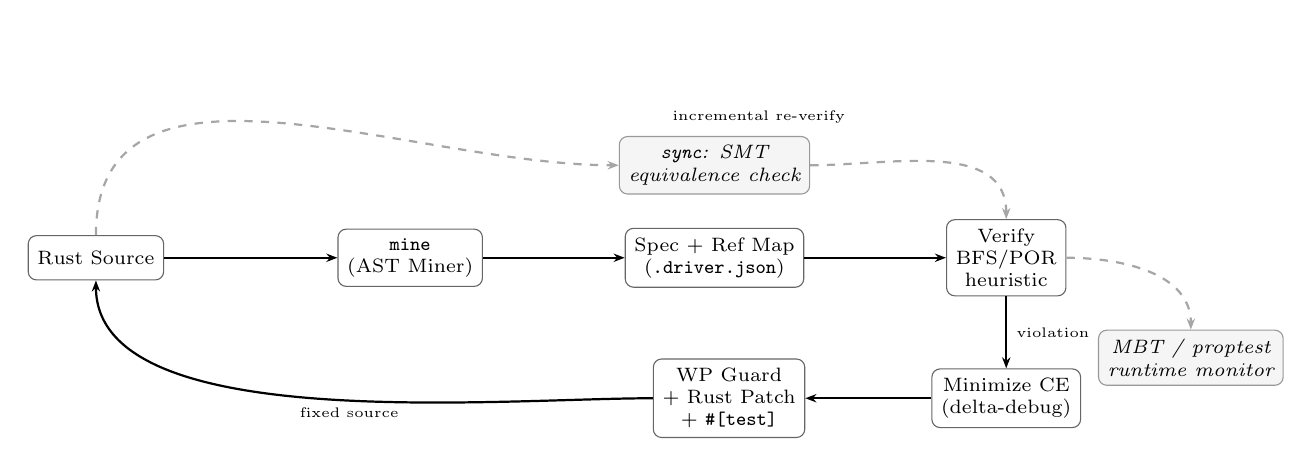
\begin{tikzpicture}[node distance=1.0em and 1.6em]
  %% === Main left-to-right pipeline ===
  \node[box]                    (rust)  {Rust Source};
  \node[box, right=2.2cm of rust]  (mine)  {\texttt{mine}\\(AST Miner)};
  \node[box, right=1.8cm of mine]  (spec)  {Spec + Ref Map\\(\texttt{.driver.json})};
  \node[box, right=1.8cm of spec]  (verify){Verify\\BFS/POR\\heuristic};

  %% === Clean (right-bottom) branch ===
  \node[sidebox, below right=1.2em and 0.4cm of verify] (assure)
        {MBT / proptest\\runtime monitor};

  %% === Violation (bottom-center) branch ===
  \node[box, below=2.6em of verify]  (min)   {Minimize CE\\(delta-debug)};
  \node[box, left=1.6cm of min]      (wp)    {WP Guard\\+ Rust Patch\\+ \texttt{\#[test]}};

  %% === Change-detection (top, dashed) ===
  \node[sidebox, above=1.2em of spec]  (sync)  {\texttt{sync}: SMT\\equivalence check};

  %% === Main arrows ===
  \draw[arr] (rust)  -- (mine);
  \draw[arr] (mine)  -- (spec);
  \draw[arr] (spec)  -- (verify);

  %% === Violation path ===
  \draw[arr] (verify) -- node[right,font=\tiny]{violation} (min);
  \draw[arr] (min)    -- (wp);

  %% Repair loop: patch → Rust source
  \draw[arr] (wp.west) to[out=180,in=270,looseness=0.7]
    node[below,font=\tiny,xshift=12pt]{fixed source} (rust.south);

  %% === Clean path ===
  \draw[darr] (verify.east) to[out=0,in=90] (assure.north);

  %% === Change-detection path ===
  \draw[darr] (rust.north) to[out=90,in=180] (sync.west);
  \draw[darr] (sync.east)  to[out=0,in=90]  (verify.north);
  \node[font=\tiny,above=0.1em of sync,xshift=16pt] {incremental re-verify};
\end{tikzpicture}}%
\caption{Spectre continuous refinement cycle.
  The \texttt{.driver.json} map (produced by \texttt{mine}) is reused by
  every downstream stage.
  The repair loop (violation $\to$ minimize $\to$ WP patch $\to$ fixed Rust)
  closes at the source level.
  The dashed change-detection path (SMT sync $\to$ incremental re-verify)
  keeps the map consistent across code evolution.}\label{fig:arch}
\end{figure}

\begin{table}[t]
\caption{Feature comparison (open-source toolchains).}\label{tab:comparison}
\centering\small
\begin{tabular}{lccc}
\toprule
Feature                              & TLA+/TLC & Quint & \textsc{Spectre} \\
\midrule
Source-derived Rust\,--\,model map  & --         & partial$^\dagger$ & \checkmark \\
SMT semantic sync / drift detection  & --         & --         & \checkmark \\
CE minimisation (delta-debugging)    & --         & --         & \checkmark \\
WP guard synthesis + Rust patch      & --         & --         & \checkmark \\
Ample-set-style POR heuristic        & $\circ^*$  & --         & \checkmark \\
Property-directed best-first search  & --         & --         & \checkmark \\
Incremental re-verification          & --         & --         & \checkmark \\
Coverage-guided MBT (5 modes)        & --         & $\circ$    & \checkmark \\
\texttt{proptest} harness gen.       & --         & --         & \checkmark \\
Runtime monitor generation           & --         & --         & \checkmark \\
Infinite-trace LTL / WF / SF        & \checkmark & \checkmark & future work \\
\bottomrule
\multicolumn{4}{l}{\small $^\dagger$Quint Connect: user-supplied state extraction required.} \\
\multicolumn{4}{l}{\small $^*$TLC provides symmetry/state-graph reduction; ample-set POR is not documented.} \\
\end{tabular}
\end{table}

% ── 3. Maintaining Refinement Under Change ────────────────────────────────────
\section{Maintaining Refinement Under Change}\label{sec:sync}

\paragraph{SMT semantic equivalence (\texttt{spectre sync}).}
\texttt{spectre sync} re-mines the Rust source and classifies each changed
guard or assignment expression.
Structural comparison catches new/renamed variables and actions but cannot
distinguish $x\!+\!n$ from $x\!-\!n$ (genuine semantic change) vs.\
$x\!>\!0$ from $\neg(x\!\le\!0)$ (logically equivalent).
Spectre encodes the query
$\exists\vec{x}.\;e_{\mathit{old}}(\vec{x})\ne e_{\mathit{new}}(\vec{x})$
in QF\_LIA and calls Z3~\cite{20_demoura2008z3}: UNSAT means equivalent; SAT
returns a distinguishing witness for the developer.

\begin{proposition}[SMT Equivalence Soundness]\label{prop:smt}
If the QF\_LIA query is UNSAT, then $e_{\mathit{old}}$ and $e_{\mathit{new}}$
are identical for all integer/Boolean valuations.
Any SAT witness is a \emph{distinguishing valuation in the encoded domain}:
it proves expression inequivalence but need not correspond to a reachable
Rust program state.
\end{proposition}

The encoding uses no \texttt{set-logic} declaration when Boolean variables are
present (letting Z3 choose); negative literals are encoded as $(- c)$;
Boolean variables are \texttt{Bool}-sorted compared via \texttt{xor}.

\paragraph{PR / CI impact analysis (\texttt{spectre impact}).}
Given a \texttt{git diff}, Spectre maps changed Rust method names to affected
spec actions, identifies invariants referencing those actions' write-sets, and
reports which invariants need re-verification.
Output gates CI pipelines: exit~1 on any non-preserving semantic change.

\paragraph{Cached and incremental verification.}
Spectre SHA-256-hashes the spec, parameters, and interpreter version, caching
the BFS graph under \texttt{.spectre-cache/}.
A cache hit avoids all re-exploration ($47\times$ speedup on Raft:
0.265\,s vs.\ 12.4\,s cold BFS).
When \texttt{sync} flags an action as \emph{possibly-unsafe},
\texttt{verify --incremental} prunes stale transitions, recomputes reachability,
and BFS-expands newly reachable states within the original bound.

\begin{proposition}[Incremental Equivalence]\label{prop:incremental}
Let $\mathcal{C}$ be a fixed exploration configuration (initial state,
parameters, depth/state bounds, action order, interpreter semantics) and
$G_{\mathcal{C}}(S)$ the graph produced under $\mathcal{C}$.
If $S'$ differs from $S$ only in action $A$'s transition relation,
incremental re-verification under $\mathcal{C}$ yields $G_{\mathcal{C}}(S')$.
\end{proposition}

\paragraph{Partial-order reduction.}
Spectre applies a conservative ample-set-style POR
heuristic~\cite{9_holzmann2003spin}: two actions are \emph{independent} if
their read/write variable sets are disjoint; if one action is independent
of all others it is explored alone, otherwise the full enabled set is used.
We validate POR results against full BFS where feasible; empirically,
POR reduces the 3-node Raft model from 22{,}432 to 6{,}818 states
($7.6\times$ speedup) and processes 5-node Raft $6.9\times$ faster at the
50{,}000-state bound.

\paragraph{Property-directed best-first search.}
Each state is assigned a \emph{linear predicate distance} to the nearest
invariant violation:
$d(e\ge c)=\max(0,c-e)$, $d(e>c)=\max(0,c-e-1)$,
$d(e\le c)=\max(0,e-c)$, $d(e<c)=\max(0,e-c-1)$,
$d(I_1\wedge I_2)=d(I_1)+d(I_2)$, $d(I_1\vee I_2)=\min(d(I_1),d(I_2))$.
States are dequeued by ascending distance; the frontier prioritises states
nearest invariant boundaries.

% ── 4. From Counterexample to Rust Repair ─────────────────────────────────────
\section{From Counterexample to Rust Repair}\label{sec:repair}

\paragraph{Counterexample minimisation.}
Given a violation trace of length $\ell$, Spectre applies Zeller's ddmin
algorithm~\cite{26_zeller2002simplifying} to find a \emph{1-minimal}
sub-sequence: removing any single step destroys the violation.
Each candidate subsequence is re-executed from the original initial state
under the model's transition semantics; it is retained only if every remaining
action is still enabled and the violation still occurs.
Path reconstruction uses a linear forward scan through original transitions
(preserving relative order after removals), avoiding positional mismatch
when the same action appears multiple times.

\paragraph{WP synthesis.}
For invariant $I$ and action $A$ with simultaneous assignments
$\{x_1'=e_1,\ldots,x_n'=e_n\}$, the weakest precondition is computed
by syntactic substitution~\cite{7_dijkstra1976discipline}:
\[
\mathrm{wp}(A,I)=I[\,x_1\leftarrow e_1,\;\ldots,\;x_n\leftarrow e_n\,]
\]

\begin{proposition}[Substitution Soundness]\label{prop:wp}
For any pre-state $\sigma$ in which $A$ is enabled:
$\sigma\models\mathrm{wp}(A,I)$ implies $A(\sigma)\models I$.
This holds for all assignment forms (arithmetic, Boolean, enum) with no
grammar search.
\end{proposition}

Algorithm~\ref{alg:wp} shows the CEGIS loop: a CE identifies the failing
$(A,I)$ pair; $\mathrm{wp}(A,I)$ is computed \emph{once} by syntactic substitution
(no grammar, no search), yielding a safety repair (invariant preserved; intended
semantics not necessarily restored); if re-verification yields a new $(A',I')$,
the procedure recurses on the already-repaired model---guards from earlier
iterations remain installed.

\begin{algorithm}[t]
\caption{$\textsc{SynthesiseGuard}(I,\,A)$}\label{alg:wp}
\begin{algorithmic}[1]
\Require Invariant $I$; action $A$ with simultaneous assignments $\{x_i'=e_i\}$
\Ensure \texttt{require} guard $g$ sufficient to block the violation
\State $g\leftarrow I[\,x_1\leftarrow e_1,\;\ldots,\;x_n\leftarrow e_n\,]$
\State Simplify $g$; add as \texttt{require} to $A$; re-explore
\If{new violation with failing pair $(A',I')$}
  \Return $\textsc{SynthesiseGuard}(I',A')$
\EndIf
\State \Return $g$
\end{algorithmic}
\end{algorithm}

\paragraph{Rust patch generation.}
The synthesised guard $g$ is translated to Rust via the refinement map:
spec variable $v$ maps to \texttt{self.\emph{rust\_field}} for state variables
and to the local parameter name for action arguments.
Operator precedence is respected (right-operand wrapping for \texttt{-} and
\texttt{/}).
If the refinement map marks the method as returning \texttt{Result}, the patch
emits \texttt{if !(\emph{g}) \{ return Err(\ldots); \}};
otherwise \texttt{assert!(\emph{g})}.

\paragraph{Generated regression test.}
The 1-minimal CE trace is serialised as ITF JSON and
\texttt{spectre verify --emit-rust-tests} produces a compilable
\texttt{\#[test]} reproducing the fault.
After the patch is applied, \texttt{spectre verify --incremental}
confirms the invariant holds.

% ── 5. Generated Conformance and Runtime Assurance ────────────────────────────
\section{Generated Conformance and Runtime Assurance}\label{sec:conformance}

All outputs below are derived from the same \texttt{.driver.json} map.

\paragraph{Coverage-guided MBT.}
\texttt{spectre verify --emit-traces --coverage-mode} generates ITF traces
in five modes: \emph{action} (prefer unseen actions),
\emph{transition-pair} (prefer unseen $(A_{\mathit{prev}},A_{\mathit{curr}})$ pairs),
\emph{boundary} (steer toward integer variable min/max),
\emph{rare-action} (prefer least-frequently-taken transitions), and
\emph{property-directed} (minimise linear predicate distance to invariant
boundary).
Traces are replayed against live Rust via the generated \texttt{StepHandler} driver.

\paragraph{Proptest, differential conformance, and runtime monitors.}
\texttt{spectre verify --emit-proptest} translates \texttt{require} guards
into \texttt{prop\_assume!} filters and invariants into \texttt{prop\_assert!}.
\texttt{spectre diff-conformance} replays one ITF trace against two spec
versions, surfacing steps where verdicts diverge.
\texttt{spectre generate-monitor} produces a self-contained \texttt{monitor.rs}
checking all invariant predicates in $O(k)$ time with no heap allocation
(3.7--6.1\,ns per check on Apple M3 Pro, $k$\,=\,1--20 clauses).

% ── 6. Evaluation ─────────────────────────────────────────────────────────────
\section{Evaluation}\label{sec:eval}

\noindent\textbf{Platform.}
Apple M3 Pro (\texttt{aarch64}), 18\,GB RAM, macOS~15.6, Go~1.24.
Default limits: 5{,}000 states / depth~100 unless noted.
All benchmarks are in \texttt{examples/}; a Docker image and
\texttt{artifact/reproduce.sh} enable reproduction.
Absolute wall times are hardware-dependent; speedup ratios (BFS/POR,
cold/warm, full/incremental) are the primary claims and are
reproducible on any platform within normal variance.

We evaluate four research questions:
\textbf{RQ1}~Raft complete lifecycle (derivation, scalability, POR, repair);
\textbf{RQ2}~semantic sync ablation (structural vs.\ AST vs.\ SMT);
\textbf{RQ3}~end-to-end repair across defect classes;
\textbf{RQ4}~spec mining breadth and guided-exploration effectiveness.

\subsection{RQ1 --- Raft: Complete Lifecycle on a Distributed Protocol}
\label{sec:eval:raft}

\paragraph{Complete lifecycle.}
We drive the entire Spectre lifecycle on Raft in a single continuous thread:
\begin{enumerate}[leftmargin=1.4em,itemsep=0pt,parsep=0pt]
\item[\textbf{(1)}] \textbf{Derive.}
  \texttt{spectre mine raft.rs} extracts a per-node skeleton
  (5 vars, 5 action types: \texttt{startElection}, \texttt{grantVote},
  \texttt{becomeLeader}, \texttt{appendEntry}, \texttt{stepDown})
  and a \texttt{.driver.json} in one pass.
\item[\textbf{(2)}] \textbf{Parameterise.}
  Three composed instances form the 3-node cluster spec (15 vars, 27 actions);
  5-node (25/75) and 7-node (35/147) follow the same pattern.
\item[\textbf{(3)}] \textbf{Verify + POR heuristic.}
  Exhaustive BFS of the 3-node cluster finds no violations in 22{,}432 states.
  POR heuristic reduces to 6{,}818 states ($7.6\times$ speedup).
\item[\textbf{(4)}] \textbf{Incremental.}
  Cache warm re-run: 0.265\,s ($47\times$); per-action incremental: $4.3$--$5.2\times$.
\item[\textbf{(5)}] \textbf{Inject fault.}
  Wrong quorum (\texttt{votes1 >= 1}); BFS detects \emph{leaderMajority} violation.
\item[\textbf{(6)}] \textbf{Minimize CE.}
  Delta-debugging confirms the trace is already 1-minimal (2 steps).
\item[\textbf{(7)}] \textbf{Diagnose.}
  Relevant vars: \texttt{state1, votes1}; first divergence at step~1.
\item[\textbf{(8)}] \textbf{WP repair.}
  Guard synthesised: \texttt{votes1 * 2 > 3}.
\item[\textbf{(9)}] \textbf{Rust patch.}
  Patch: \texttt{assert!(self.votes * 2 > 3)}; compiles without error.
\item[\textbf{(10)}] \textbf{Regression test.}
  Minimised CE serialised as \texttt{\#[test]}; passes after patch applied.
\item[\textbf{(11)}] \textbf{Re-verify.}
  \texttt{spectre verify --incremental} confirms invariant holds.
  Total end-to-end time (detect $\to$ re-verify): 1.6\,s.
\item[\textbf{(12)}] \textbf{Semantic drift + safety repair.}
  Second fault: \texttt{term1' = term1} (missing \texttt{+\,1}).
  \texttt{spectre sync} flags genuine drift; 6-step CE violates
  \emph{electionSafety}.
  WP guard: \texttt{term1 != term2 \&\& term1 != term3}---a
  \textbf{safety repair}: restricts executions to preserve the invariant
  but does not restore the missing increment; \texttt{diff-conformance} flags
  over-restriction. The underlying bug requires a code fix, not a guard.
\item[\textbf{(13)}] \textbf{Scale.}
  5-node BFS: ${>}50{,}000$ states in 268\,s ($6.9\times$ faster with POR: 38.7\,s);
  reachable space exceeds the 50{,}000-state bound---simulation provides coverage
  (100 traces, 0.56\,s).
  7-node: simulation only (100 traces, 1.64\,s).
\end{enumerate}
Terms and log lengths are bounded 0--3; this is a finite abstraction of the
election sub-protocol, not full Raft verification.
Tables~\ref{tab:raft-scale}--\ref{tab:raft-repair} report detailed measurements.

\begin{table}[t]
\caption{Raft scalability. $^\dagger$ State limit reached; full reachable-state count not determined.
  5-node POR heuristic is $6.9\times$ faster than BFS at the same budget.}\label{tab:raft-scale}
\centering\small
\begin{tabular}{lrrrrr}
\toprule
Config & Vars & Actions & States explored & Time & Sim (100 traces) \\
\midrule
3-node BFS  & 15 & 27 & 22{,}432             & 12.4\,s & -- \\
3-node POR  & 15 & 27 & 6{,}818             & 1.63\,s & -- \\
5-node BFS  & 25 & 75 & ${>}50{,}000^\dagger$ & 268\,s  & 0.56\,s \\
5-node POR  & 25 & 75 & ${>}50{,}000^\dagger$ & 38.7\,s & -- \\
7-node      & 35 & 147& not attempted        & --      & 1.64\,s \\
\bottomrule
\end{tabular}
\end{table}

\smallskip

\begin{table}[t]
\caption{Incremental re-verification on 3-node Raft (cold BFS 12.4\,s).
  \emph{Pruned} = states removed as unreachable without the changed action.}\label{tab:raft-incr}
\centering\small
\begin{tabular}{lrrrc}
\toprule
Changed action & Incremental & Speedup & Pruned & New BFS \\
\midrule
\texttt{stepDown1\_s2} & 2.4\,s & $5.2\times$ & 1{,}649 & ${\approx}$1{,}644 \\
\texttt{vote2for1}     & 2.9\,s & $4.3\times$ & 6{,}501 & ${\approx}$6{,}493 \\
\bottomrule
\end{tabular}
\end{table}

\smallskip

\begin{table}[t]
\caption{End-to-end repair on injected Raft faults.
  CE/Min = trace length (original / 1-minimal).
  $^\dagger$Safety repair: guard restricts executions to preserve the invariant
  but does not restore the missing \texttt{term+1} assignment;
  \texttt{diff-conformance} detects over-restriction.}\label{tab:raft-repair}
\centering\small
\begin{tabular}{lrrlcc}
\toprule
Injected fault & CE & Min & WP guard & Patch & Test \\
\midrule
Wrong quorum    & 2 & 2 & \texttt{votes1*2 > 3}  & \checkmark & \checkmark \\
Missing term incr.$^\dagger$& 6 & 6 & \texttt{term1$\ne$term2 $\wedge$ term1$\ne$term3} & \checkmark$^\dagger$ & \checkmark \\
\bottomrule
\end{tabular}
\end{table}

\subsection{RQ2 --- Semantic Synchronisation Ablation}\label{sec:eval:sync}

\paragraph{Setup.}
We construct two corpora from the \texttt{bank\_account} Rust component:
(a)~8 genuine semantic mutations (wrong operator, wrong comparison, polarity
inversion, guard omission);
(b)~5 semantics-preserving transformations (commutativity, constant folding,
double negation, guard reordering).
We compare three methods: field/action count only (\emph{Structural});
normalised AST string matching (\emph{Norm.~AST});
and \emph{AST + SMT} (our approach).

\begin{table}[t]
\caption{Semantic sync ablation (8 semantic mutations + 5 equivalent rewrites).
  FP~=~false positives (equivalent edits flagged); FN~=~false negatives
  (semantic changes missed).}\label{tab:sync}
\centering\small
\begin{tabular}{lcccc}
\toprule
Method & Semantic detected & Equiv.\ accepted & FP & FN \\
\midrule
Structural      & 3 / 8 & 5 / 5 & 0 & 5 \\
Normalised AST  & 8 / 8 & 1 / 5 & 4 & 0 \\
AST + SMT       & 8 / 8 & 4 / 5 & 1 & 0 \\
\bottomrule
\end{tabular}
\end{table}

Structural comparison detects only count-level changes (3/8 semantic),
missing arithmetic mutations.
Normalised AST detects all semantic changes but rejects 4/5 equivalent
rewrites (high FP).
AST + SMT detects all 8 semantic mutations with only 1 FP
(guard reordering, a known limitation of positional matching)---a clear
win over both baselines.

\subsection{RQ3 --- End-to-End Repair}\label{sec:eval:repair}

We apply the full seven-stage pipeline---CE, minimize, WP, patch, compile,
\texttt{\#[test]}, re-verify---to one representative defect per class.

\begin{table}[t]
\caption{End-to-end repair pipeline across defect classes.
  CE/Min = original / minimised trace length;
  $\surd$ = stage succeeded; -- = stage not reached.}\label{tab:repair}
\centering\scriptsize
\begin{tabular}{lrrccccc}
\toprule
Spec & CE / Min & WP guard & WP & Patch & Compile & Test & Reverify \\
\midrule
\texttt{repair-arith}       & 1/1 & \texttt{balance - amount >= 0} & $\surd$ & $\surd$ & $\surd$ & $\surd$ & $\surd$ \\
\texttt{repair-bool}        & 1/1 & \texttt{!(active = true)}      & $\surd$ & $\surd$ & $\surd$ & $\surd$ & $\surd$ \\
\texttt{repair-enum}        & 1/1 & \texttt{status != Running}      & $\surd$ & $\surd$ & $\surd$ & $\surd$ & $\surd$ \\
\texttt{repair-simultaneous}& 4/1 & \texttt{balance - 30 >= 0}      & $\surd$ & $\surd$ & $\surd$ & $\surd$ & $\surd$ \\
\texttt{repair-protocol}    & 2/2 & (missing upstream guard)        & --      & --      & --      & --      & -- \\
\midrule
\textbf{Total}              &     &                                 & 4/5 & 4/5 & 4/5 & 4/5 & 4/5 \\
\bottomrule
\end{tabular}
\end{table}

The unsynthesisable case (\texttt{repair-protocol}) illustrates a known
limitation: the \emph{missing readiness guard} requires WP reasoning across
two actions (the setter and the consumer); single-action WP cannot express it.
This is a precise boundary, not a random failure, and is future work.

\subsection{RQ4 --- Spec Mining and Directed Testing}\label{sec:eval:external}

\paragraph{Mining breadth within the supported Rust subset.}
We measure construct diversity (not yet external validity) by applying
\texttt{spectre mine} to 9 author-written Rust components spanning five
design archetypes: bounded resource managers (semaphore, connection pool),
FIFO/LIFO collections (queue, stack), event-driven structures (event log),
finite-state machines (circuit breaker), and key/value stores (cache, bank
account, rate limiter).
All 9 produce parseable, type-correct specs with zero manual edits---100\%
field/action yield across primitive types (\texttt{int}, \texttt{bool}, \texttt{enum}).
All nine mined specifications parse, type-check, and execute under Spectre
without manual modification.
Evaluation on independent open-source crates is left to future work.

\begin{table}[t]
\caption{Mining breadth: 9 Rust components, 100\% automatic yield.
  $^\dagger$ BFS bounded at 5{,}000 states.}\label{tab:external}
\centering\small
\begin{tabular}{lrrrrl}
\toprule
Component & LOC & Fields & Actions & Guards & BFS / time \\
\midrule
\texttt{cache}            & 13 & 4 & 4 & 1  & ${\geq}5{,}000^\dagger$ / 0.35\,s \\
\texttt{rate\_limiter}    & 11 & 3 & 3 & 3  & 1 / ${<}0.01$\,s \\
\texttt{bank\_account}    & 30 & 3 & 4 & 7  & 3{,}745 / 1.70\,s \\
\texttt{queue}            & 12 & 4 & 3 & 2  & 1 / ${<}0.01$\,s \\
\texttt{circuit\_breaker} & 14 & 4 & 4 & 5  & 5 / ${<}0.01$\,s \\
\texttt{stack}            & 11 & 3 & 3 & 2  & 2 / ${<}0.01$\,s \\
\texttt{semaphore}        & 12 & 3 & 4 & 4  & 2{,}550 / 0.07\,s \\
\texttt{event\_log}       & 14 & 4 & 5 & 6  & 2 / ${<}0.01$\,s \\
\texttt{connection\_pool} & 12 & 3 & 4 & 4  & 1 / ${<}0.01$\,s \\
\bottomrule
\end{tabular}
\end{table}

Generic or \texttt{unsafe} Rust requires additional manual abstraction beyond
the current miner's scope.

\paragraph{Guided exploration vs.\ random simulation (RQ4b).}
A 5-action seeded-fault spec requires 6 consecutive \texttt{inc} steps;
3 distractor and 1 reset actions suppress random walks.

\begin{table}[t]
\caption{Systematic search finds all 29 distinct violation-reaching traces after
  204 explored states; random simulation finds none in 150{,}000 steps
  (5{,}000 runs $\times$ 30 steps, seeds 1--5{,}000). PD = property-directed.}\label{tab:testing}
\centering\scriptsize
\begin{tabular}{lrrl}
\toprule
Strategy & Budget & Violations & States / steps explored \\
\midrule
BFS              & 50{,}000 states & 29 & 204 states \\
PD (\texttt{--property-guided}) & 50{,}000 states & 29 & 204 states \\
Random ($\le$5{,}000$\times$30) & 150{,}000 steps & 0  & 150{,}000 steps \\
\bottomrule
\end{tabular}
\end{table}

Both systematic strategies find all 29 distinct violation-reaching traces after
204 explored states; none of the 5{,}000 independent 30-step random simulations
finds even one.

% ── 7. Related Work ───────────────────────────────────────────────────────────
\section{Related Work}\label{sec:related}

\paragraph{Specification-first tools.}
TLA+/TLC~\cite{16_lamport2002specifying,15_kuppe2019toolbox} and Quint~\cite{12_informal2023quint}
require user-authored models.
Quint Connect~\cite{13_informal2024quintconnect} and tla\_connect~\cite{2_tlaconnect2024} provide
Rust MBT and ITF replay bridges, but state extraction and step mapping are
user-supplied.
C\^{i}rstea et al.~\cite{4_cirstea2024validating} validate distributed program traces
against TLA+ specs; Maliuginas and Petrauskas~\cite{19_maliuginas2024extracting}
extract TLA+ from a BEAM virtual machine program.
Spectre pursues the complementary \emph{implementation-first} direction:
derivation, synchronisation, repair, testing, and monitoring are all driven
by a single source-derived refinement correspondence.

\paragraph{Annotation-based, deductive, and synthesis tools.}
Ivy~\cite{22_padon2016ivy} and Dafny~\cite{18_leino2010dafny} rely on
user-authored formal specifications rather than deriving a Rust--model
correspondence from existing source.
P~\cite{6_desai2013p} unifies implementation and systematic testing in a
dedicated event-driven language; Spectre operates on existing idiomatic Rust.
CEGIS~\cite{24_solarlezama2008program} iteratively refines candidates using
counterexamples; SyGuS~\cite{1_alur2013sygus} additionally constrains candidates
via a syntactic grammar. Spectre's candidate guard is instead computed directly
by WP substitution and translated back to Rust via the refinement map.
Verus~\cite{17_lattuada2023verus} verifies Rust via user-authored ghost-type
annotations; ExVerus~\cite{25_yang2026exverus} adds CE-guided proof repair.
Spectre requires no inline proof annotations or proof obligations; correctness
invariants remain independently supplied by the user.

\paragraph{Model extraction, invariant inference, and runtime verification.}
SPIN/Modex~\cite{9_holzmann2003spin,10_holzmann2001modex} extract Promela from C;
Spectre targets Rust and additionally reuses the correspondence for repair,
testing, and monitoring.
Daikon~\cite{8_ernst2007daikon} infers invariants dynamically; Spectre generates
candidates requiring explicit human acceptance.
MOP/JavaMOP~\cite{3_chen2007mop,14_jin2012javamop} use separate monitor DSLs;
Spectre derives monitors from the same spec.
ITF traces~\cite{11_informal2022itf} are the interchange standard.

% ── 8. Conclusion ─────────────────────────────────────────────────────────────
\section{Conclusion}\label{sec:conclusion}

\textsc{Spectre} demonstrates that a source-derived refinement map can serve
as persistent verification infrastructure across the Rust development lifecycle.
The central thesis---that the refinement relation should be derived once and
maintained, not rebuilt per tool---is validated by showing the same
\texttt{.driver.json} artifact driving semantic sync, incremental verification,
CE minimisation, WP patch generation, MBT trace replay, proptest harnesses,
and runtime monitors.
The Raft case study demonstrates the complete system: 22{,}432-state exhaustive
verification, $7.6\times$ POR heuristic speedup, $47\times$ cache speedup,
incremental re-verification ($4.3$--$5.2\times$ speedup), and end-to-end fault repair.
Limitations: bounded checking; no infinite-trace LTL; external-crate mining
requires manual abstraction for generic/unsafe Rust.
The tool, artifact, and Docker image are at
\url{https://github.com/BoundlessProducts/spectre};
a Zenodo DOI will accompany the camera-ready version.

% ── References ────────────────────────────────────────────────────────────────
\bibliographystyle{splncs04}
\bibliography{references}

\end{document}
